\noindent In perturbative, interacting field theories, we must calculate the $n$-point correlation function
\begin{equation}
G^{(n)}(x_1,\dots,x_n) = \frac{\bra{0} \mathcal{T} [\hat{\phi}_1 \dots \hat{\phi}_n \mathcal{S}]\ket{0}}{\bra{0} \mathcal{S} \ket{0}}
\end{equation}

\noindent Where the scattering matrix elements and the interacting Hamiltonian are
\begin{align}
\bra{\phi} \mathcal{S} \ket{\psi} &= \lim_{t\to\infty} \bra{\phi} \mathcal{T}[e^{-i\int^t_{-t} \hat{H}_I(t')dt'}] \ket{\psi} \\
\hat{H}_I(t) &= \frac{\lambda}{4!} \int d^3 x \,\hat{\phi}^4(\textbf{x})
\end{align}

\noindent The numerator and denominator of the correlation function must be expanded perturbatively in the small parameter $\lambda$. 
\begin{align}
G^{(n)} &= \frac{a_0 + \lambda a_1 + \lambda^2 a_2 + \dots}{b_0 + \lambda b_1 + \lambda^2 b_2 + \dots} \text{, where } a_j, b_j \in \mathbb{C} \\
&= \frac{1}{b_0} (a_0 + \lambda a_1 + \dots) (1 - \lambda \frac{b_1}{b_0} + \lambda^2 \frac{b_2}{b_0} + \dots) \\
&=_{\mathcal{O}(\lambda)} \frac{1}{b_0} (a_0 + \lambda a_1) (1-\lambda \frac{b_1}{b_0}) \\
G^{(n)} &= \frac{a_0}{b_0} + \lambda (\frac{a_1}{b_0} - \frac{b_1 a_0}{b_0^2}) \text{ to order } \lambda
\end{align}

\noindent This gives the intermediate task of calculating the coefficients of the perturbative expansion: $a_0$, $a_1$, $b_0$, and $b_1$. \\

\noindent Consider the $n=2$ case
\begin{equation}
G^{(2)}(x, y) = \lim_{t\to\infty} \frac{\bra{0} \mathcal{T} [\hat{\phi}(x) \hat{\phi}(y) e^{-i\int^t_{-t} \hat{H}_I(t')dt'}]\ket{0}}{\bra{0} \mathcal{T}[e^{-i\int^t_{-t} \hat{H}_I(t')dt'}]\ket{0}}
\end{equation}

\noindent Expand the exponentials, keeping to order $\lambda$, and insert into numerator. The numerator is then
\begin{align}
\bra{0} \mathcal{T} [\hat{\phi}(x) \hat{\phi}(y) \mathcal{S}]\ket{0} &= \bra{0} \mathcal{T} [\hat{\phi}(x) \hat{\phi}(y) e^{-i\int^t_{-t} \hat{H}_I(t')dt'}]\ket{0} \\
&= \bra{0} \mathcal{T} [\hat{\phi}(x) \hat{\phi}(y) \left( \mathbb{I} - \frac{i\lambda}{4!} \int d^4 z \, \hat{\phi}^4(z) \right)]\ket{0} \\
&= \bra{0} \mathcal{T} [\hat{\phi}(x) \hat{\phi}(y)] \ket{0} - \frac{i\lambda}{4!} \int d^4 z \, \bra{0} \mathcal{T} [\hat{\phi}(x) \hat{\phi}(y) \hat{\phi}^4(z)] \ket{0} \\
\bra{0} \mathcal{T} [\hat{\phi}(x) \hat{\phi}(y) \mathcal{S}]\ket{0} &= \Delta_F(x-y) - \frac{i\lambda}{4!} \int d^4 z \, \bra{0} \mathcal{N} [\hat{\phi}(x) \hat{\phi}(y) \hat{\phi}^4(z) + \text{all contractions}] \ket{0}
\end{align}

\noindent The last line is gotten by applying Wick's theorem, and recall that any terms with \textit{uncontracted} operators will evaluate to \textbf{zero} in the vacuum expectation value (e.g., $\bra{0}\mathcal{N}[\dots]\ket{0}$), and only the \textit{fully contracted} terms will contribute, such as $\bra{0}\wick[offset=1.5em]{\c1 {\hat{\phi}(x)} \c2 {\hat{\phi}(y)} \c3 {\hat{\phi}(z)} \c2 {\hat{\phi}(z)} \c1 {\hat{\phi}(z)} \c3 {\hat{\phi}(z)}}\ket{0}$, and $\bra{0}\wick[offset=1.5em]{\c1 {\hat{\phi}(x)} \c1 {\hat{\phi}(y)} \c2 {\hat{\phi}(z)} \c2 {\hat{\phi}(z)} \c3 {\hat{\phi}(z)} \c3 {\hat{\phi}(z)}}\ket{0}$. \\

\noindent Now, "all good physics and math ends in linear algebra, combinatorics, or both", and we use combinatorics to calculate how many fully contracted terms we expect to see in the expansion. 
\begin{itemize}
\item There are $(2n-1)!!$ full contractions per expansion, where $n$ is the number of unique particles. In this case, $n=3$ for $x$, $y$, and $z$ spacetime coordinates.
\item There are 2 unique contraction types out of the $(2\cdot3-1)!! = 15$ full contractions.
	\subitem $\Delta_F(x-y) \Delta_F^2(z-z)$
	\subitem $\Delta_F(x-z) \Delta_F(y-z) \Delta_F(z-z)$
\item There are 3 contractions of the first type
	\subitem Connect $x\to y$ in 1 way and $z\to z$ twice, each in only 1 way.
\item There are 12 contractions of the second type
	\subitem Connect $x\to z$ in 4 ways, followed by $y\to z$ in 3 ways, and $4\cdot 3=12$.
\end{itemize}

\noindent Return to the numerator of the correlation function, and pretending that $\Delta_F(z-z)$ is finite, for now,
\begin{align*}
\bra{0} \mathcal{T} [\hat{\phi}(x) \hat{\phi}(y) \mathcal{S}]\ket{0} &= \Delta_F(x-y) \\
&\,\,\,\,\,\, + \left(-\frac{i\lambda}{4!}\right) \int d^4 z \, \bra{0} \mathcal{N} [\cancel{\hat{\phi}(x) \hat{\phi}(y) \hat{\phi}^4(z)} + \cancel{\text{\tiny {\stackanchor{all partial}{contractions}}}} + \text{\tiny {\stackanchor{all full}{contractions}}}] \ket{0} \\
&= \Delta_F(x-y) + 3 \cdot \left(-\frac{i\lambda}{4!}\right)\int d^4 z \, \Delta_F(x-y) \Delta_F^2(z-z) \\
&\,\,\,\,\,\, + 12 \cdot \left(-\frac{i\lambda}{4!}\right)\int d^4 z \, \Delta_F(x-z) \Delta_F(y-z) \Delta_F(z-z)
\end{align*}

\noindent And in diagrammatic form

\begin{figure}[H]
	\centering
	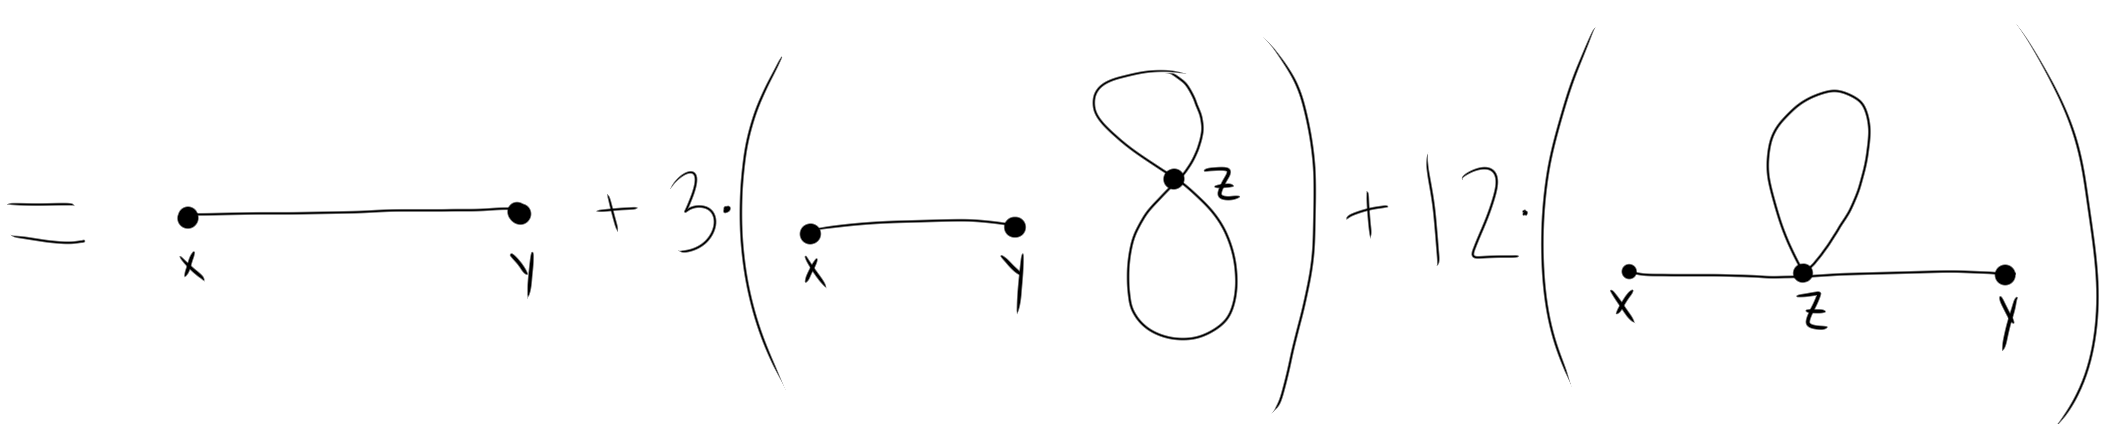
\includegraphics[scale=0.3]{feynman2.png}
	\caption{Feynman diagram representation of the above integral values for the $\varphi^4$ interacting theory.}
\end{figure}

\noindent Similarly calculate the denominator of the two-point correlation function to obtain the following

\begin{figure}[H]
	\centering
	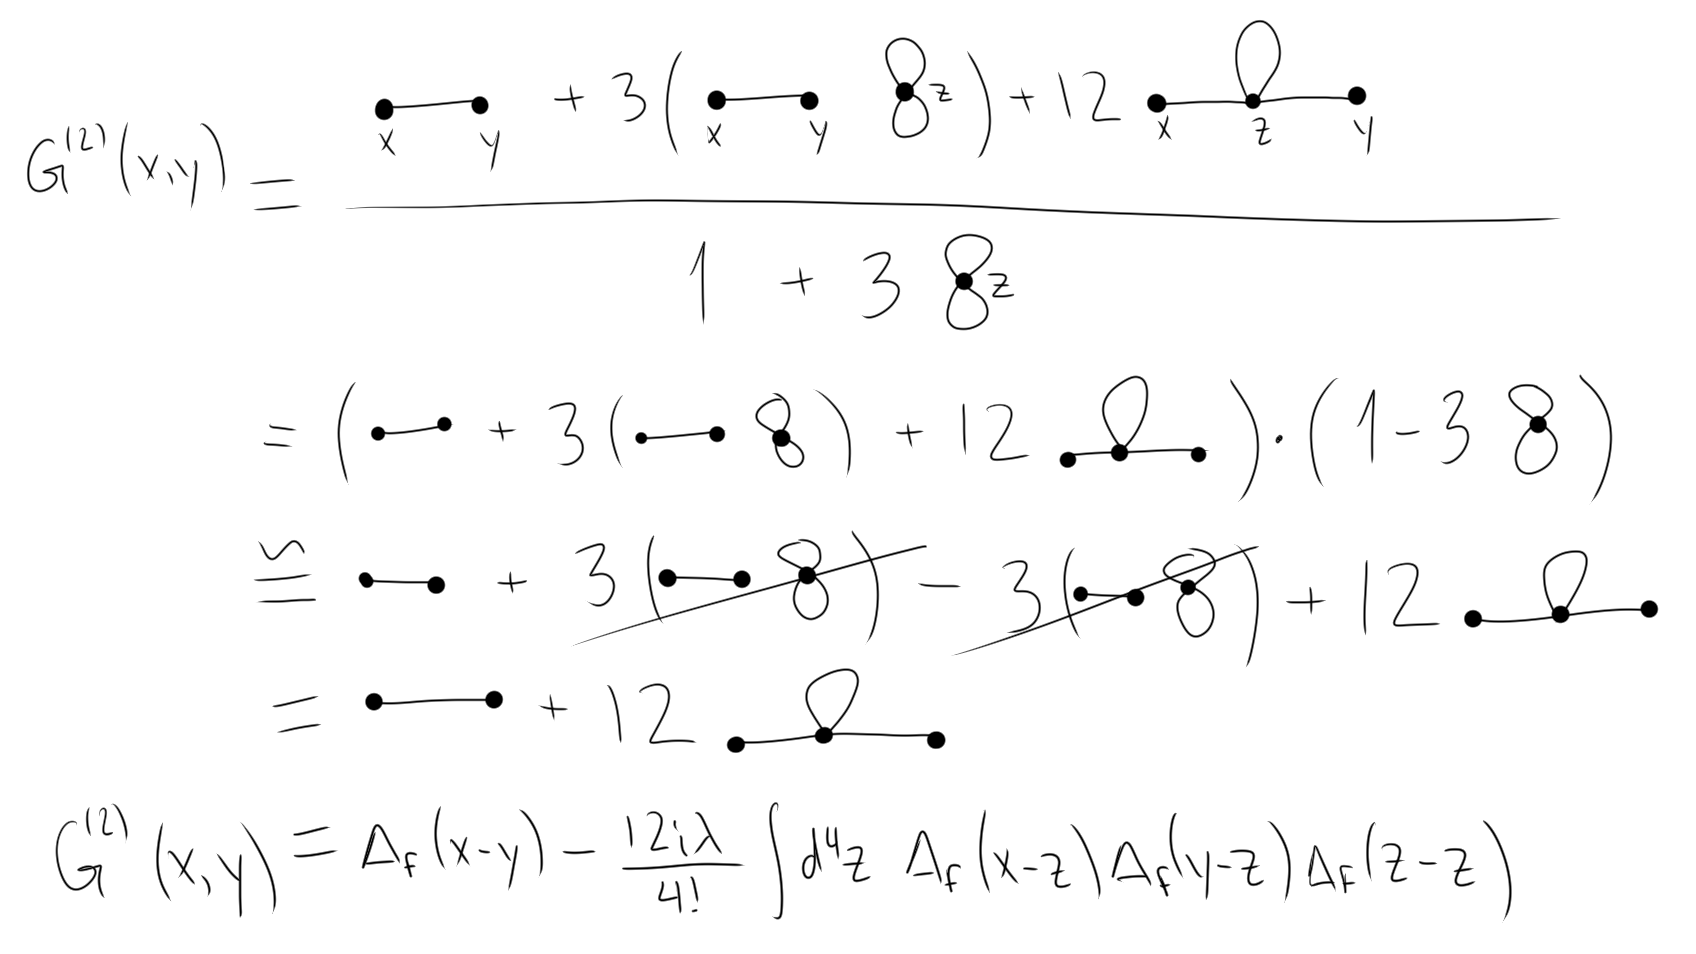
\includegraphics[scale=0.4]{twopoint.png}
	\caption{Feynman diagram calculation for the two-point correlation function for the $\varphi^4$ theory. Note that this "miraculous" cancellation of divergent terms (the "self-interacting figure-eight") actually follows from a more general result.}
\end{figure}

\noindent The arguments of the correlation function are the \textbf{external vertices}, and the spacetime coordinates of the interacting Hamiltonian are the \textbf{internal vertices}.

\noindent To calculate the value of a diagram, associate a factor, the Feynman propagator, $\Delta_F(x-y)$ to each edge connecting external vertices (e.g., $x$ and $y$), and associate the factor $-i\lambda \int d^4 z$ (dividing by the symmetry factor $4!$) to each internal vertex (e.g., $z$). \\

\noindent For example,

\begin{figure}[H]
	\centering
	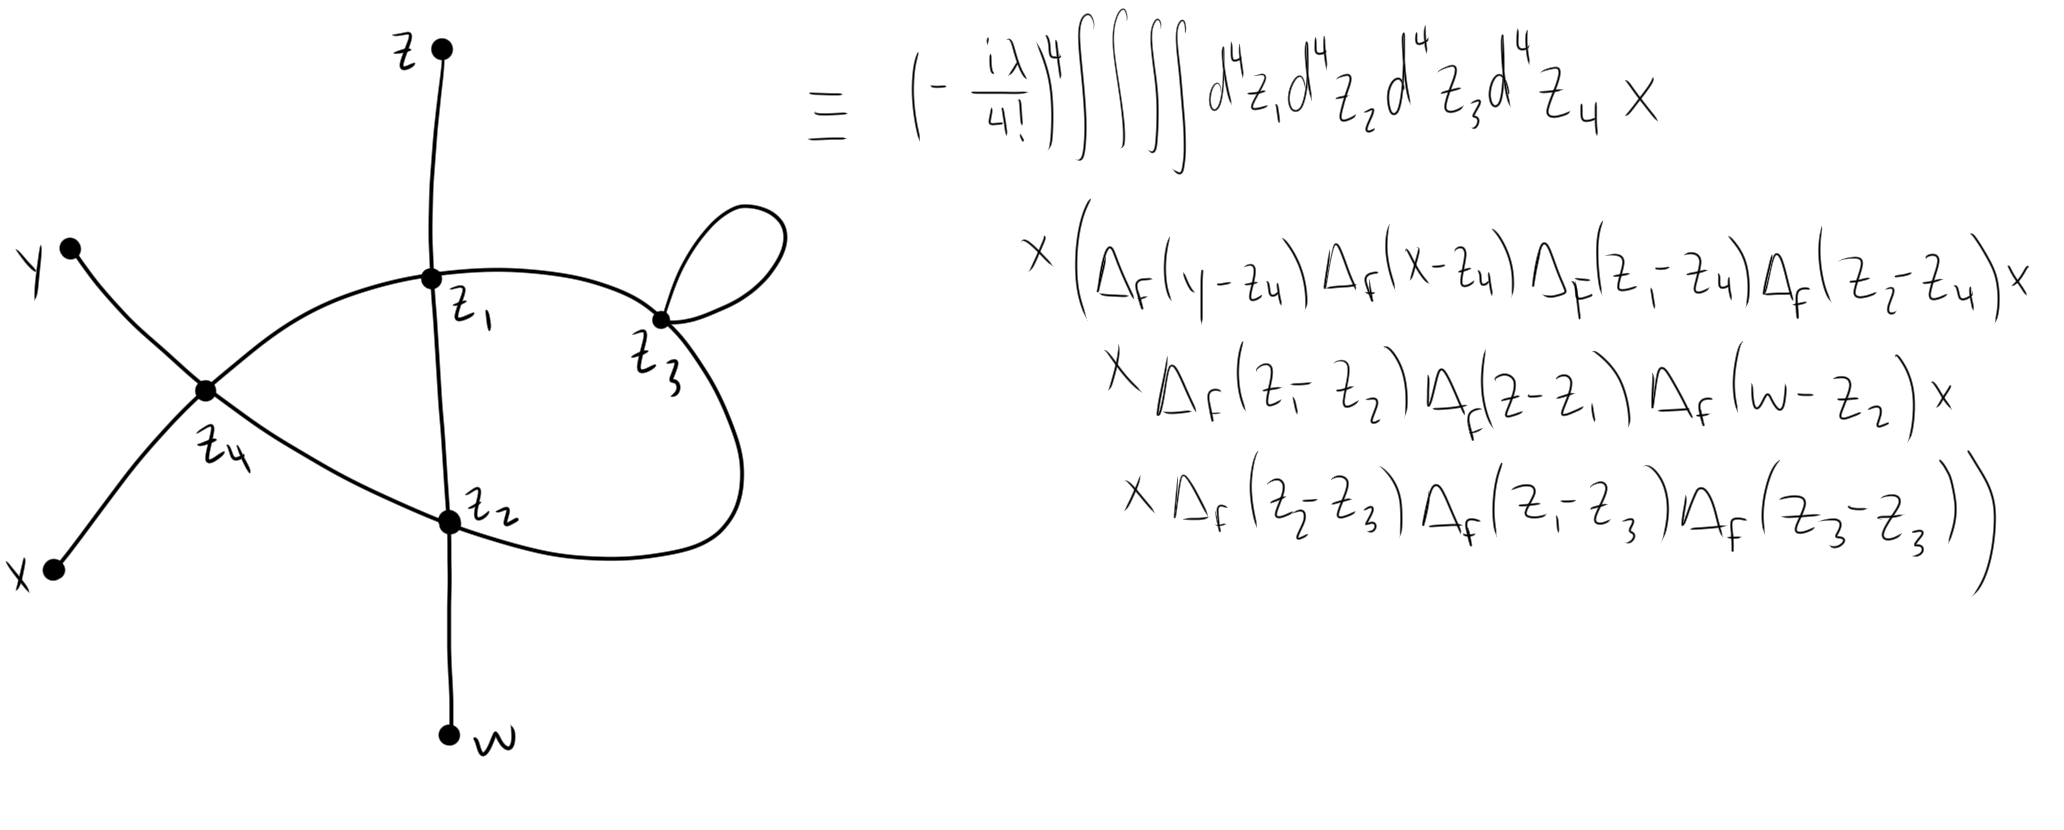
\includegraphics[scale=0.3]{4int4ext.png}
	\caption{Example Feynman diagram and associated values with 4 external vertices and 4 internal vertices.}
\end{figure}

\noindent In summary, to calculate $G^{(2)}(x,y)$ to arbitrary order, sum over all possible diagrams with 2 external vertices, subject to the (canonical) Feynman rules for $\varphi^4$ theory.

\begin{equation}
G^{(2)}(x,y) = \frac{\bra{0}\mathcal{T}[\hat{\phi}(x)\hat{\phi}(y)\mathcal{S}]\ket{0}}{\bra{0}\mathcal{S}\ket{0}} = \left(\text{\small {\stackanchor{sum of all possible diagrams}{with two external vertices}}}\right)
\end{equation}

\begin{figure}[H]
	\centering
	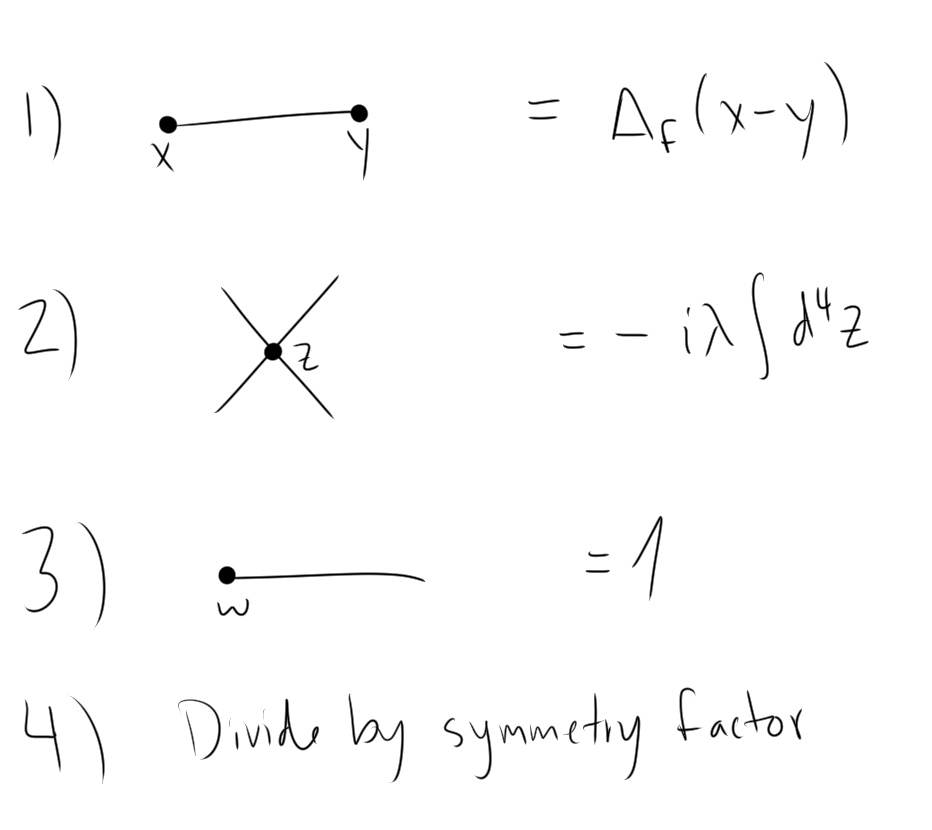
\includegraphics[scale=0.5]{phi4rules.png}
	\caption{\textbf{Canonical Feynman rules for $\varphi^4$ theory}.}
\end{figure}

\noindent Note the abscence of the inverse $4!$ factor in rule number 2, as it is added based on observation, and not considered a component on the \textit{canonical} rules. \\

\noindent Higher order terms in the expansion of the two-point correlation function become successively more complicated and often redundant. For example, The self-interacting "figure-eight" diagram of an internal vertex can occur in $4!\cdot8=192$ ways. The redundancy is encoded in the \textbf{symmetry factor} (see rule 4 above) of the diagram. Typically, in practice and computation, distinct diagrams are written down and overcounting is determined via the symmetry factor.